\chapter{Supplementary Material for Radio-Frequency methods for Majorana-Based Quantum Devices}

\section{Instruments}
\label{sec:majo_B}

Reflectometry measurements presented in Fig.~\ref{fig:majo_f} were performed with the customised demodulation circuit presented in Fig.~\ref{fig:majo_g}. Below we list other electronic equipment used in the experiments.

\begin{figure}
    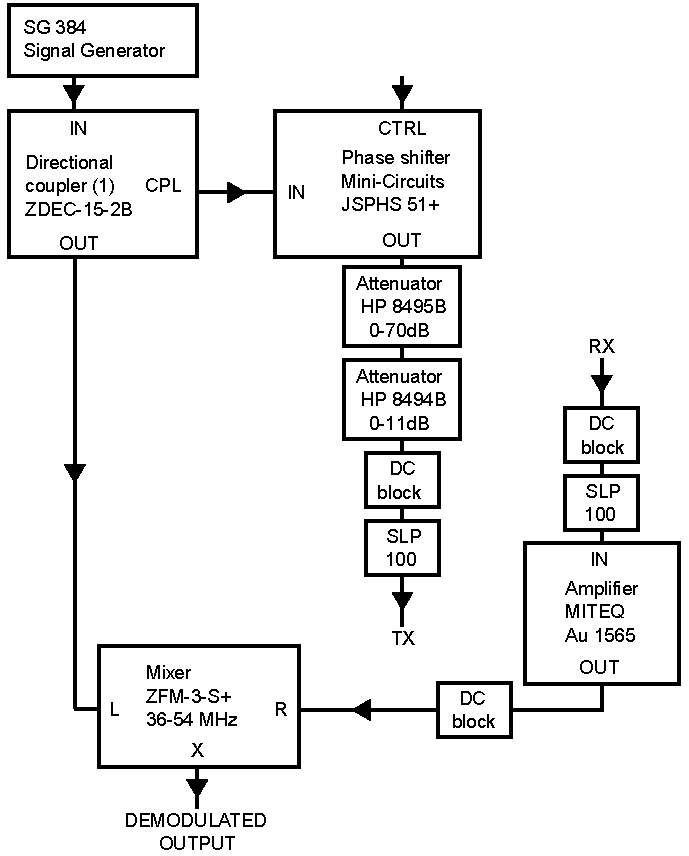
\includegraphics[width=0.48\textwidth]{Fig7-0.pdf}
      \caption[Block diagram of demodulation circuit]{Block diagram of demodulation circuit.}
      \label{fig:majo_g}
\end{figure}

\begin{enumerate}
\item Demodulation unit used for reflectometry measurements in Fig.~\ref{fig:majo_d} and Fig.~\ref{fig:majo_e}: Zurich Instruments, Ultrafast Lock-in Amplifier (\SI{600}{\mega\hertz})\footnote{Electronic Access: https://www.zhinst.com/products/uhfli}

\item Current-to-voltage converter: University of Basel, Electronics Lab, Low Noise/High stability I/V converter, SP 983 with IF3602

\item Voltage sources: 48-channel QDAC, custom digital-to-analog converters, QDevil ApS\footnote{Electronic Access: https://www.qdevil.com}

\item Lock-in: Stanford Research SR830 DSP Lock-in amplifier

\item Waveform generator: Keysight 33500B

\item Arbitrary waveform generator: Tektronix 5014 C, 1.2 GS/s

\item Vector network analyser: Rohde $\&$ Schwarz - ZVB8

\item Directional coupler: Minicircuits ZEDC-15-2B (\SI{1}{\mega\hertz} - \SI{1}{\giga\hertz})

\item Microwave switch Minicircuits ZASWA-2-50DR+ (DC - \SI{5}{\giga\hertz})

\item Cryogenic \SI{4}{\kelvin} amplifier: Caltech Weinreb CITLF3

\item Digitizer: AlazarTech ATS9360 - 12 bit, 1.8 GS/s
\end{enumerate}

\section{Signal-to-Noise Ratio and Visibility}
\label{sec:majo_C}
The extraction of signal-to-noise ratio (SNR) and visibility was accomplished with the following pulse sequence cycle [Fig.~\ref{fig:majo_e} (a) inset]. The pulse sequence starts with a fixed amplitude voltage pulse on gates $RP$ (positive voltage pulse) and $LP$ (negative voltage pulse) bringing the system to a point I for a duration of $\tau_{I} = \SI{150}{\micro\second}$ for initialization into a relative charge state $N+2$. Then, the gates $LP$ (positive voltage pulse) and $RP$ (negative voltage pulse) bring the system into a relative charge $N$ state (point P) for a time $\tau_{P} = \SI{200}{\micro\second}$. Finally, gates $LP$ (negative voltage) and $RP$ (positive voltage) bring the system close to intra-island degeneracy point M (between $N$ and $N+2$ relative charge states) which we denote as measurement position. $V_{TX}$ excitation was controlled with microwave switch (ZASWA-2-50DR+), in order to avoid disturbances in the system during the manipulation phase (I and P). The readout was performed only at the measurement point (M) by triggering the ATS9360, 12 bit waveform digitizer card for a total time duration of $\tau = \SI{50}{\micro\second}$.  To build statistics $N_\textrm{cycles} = 10^8$ experimental runs of the pulse sequence were performed. From histograms of $V^{(S2)}_{rf}$ measurements (with \SI{2}{\milli\volt} bin size), the probability, $P_{V^{(S2)}_{rf}}$ of singe-shot outcomes can be estimated for each value of measurement time $\tau$.

For the sake of simplicity, all denoted $V_\textrm{rf}$ here will refer to demodulated voltage with the right charge sensor ($V_\textrm{rf}^{(S2)}$). Visibility is defined as \cite{barthel2009rapid}:
\begin{equation}
  V = F_{N} + F_{N+2} - 1
\end{equation}
where $F_{N}$ and $F_{N+2}$ are the fidelities of relative charge state $N$ and $N+2$, respectively. The fidelity of a charge state, $N$, is defined by $F_{N} = 1 - \textrm{erf}(N)$, where $\textrm{erf}(N)$ is an probability of measuring an $N+2$ charge state when in the $N$ state. The $N+2$ state fidelity is similarly expressed as $F_{N+2} = 1 - \textrm{erf}(N+2)$. This error is calculated by evaluating cumulative normal distribution function up to the threshold voltage $V_T$, which for $N+2$ state is:
\begin{equation}
  \textrm{erf}(N+2) = \int_{-\infty}^{V_{T}}n_{N+2}(V_\textrm{rf})\textrm{d}V_{rf}
\end{equation}
where $V_{T}$ is the threshold voltage calculated from the center of the means of the two Gaussians:
\begin{equation}
  V_\textrm{rf} = \frac{\mu_{N}+\mu_{N+2}}{2}
\end{equation}
and $n_{N+2}(V_\textrm{rf})$ is the probability density function for the relative charge state $N+2$:
\begin{equation}
  n_{N+2}(V_\textrm{rf}) = \frac{e^{{(V_\textrm{rf} - \mu_{N+2})^2}/2\sigma_{N+2}^{2}}}{\sqrt{2\pi}\sigma_{N+2}}
\end{equation}

Similarly the value of $\textrm{erf}(N)$ is calculated as:
\begin{equation}
  \textrm{erf}(N) = \int_{V_{T}}^{\infty}n_{N}(V_\textrm{rf})\textrm{d}V_{rf}
\end{equation}
and $n_{N}(V_\textrm{rf})$ is the probability density function for the relative charge state $N$:
\begin{equation}
  n_{N}(V_\textrm{rf}) = \frac{e^{{(V_{\rm rf} - \mu_{N})^2}/2\sigma_{N}^{2}}}{\sqrt{2\pi}\sigma_{N}}
\end{equation}

Minimizing the function of two errors ($\textrm{erf}(N)$ and $\textrm{erf}(N+2)$) and then inserting found fidelities we calculate the visibility
\begin{equation}
  V = 1 - \textrm{erf}(N) + 1 - \textrm{erf}(N+2) - 1
\end{equation}
This yields a visibility $V = 99.8\%$ for an integration time of \SI{1}{\micro\second}.

\section{Fabrication}
\label{sec:majo_D}

All devices presented have nanowire (NW) diameter  $\sim \SI{100}{\nano\meter}$. NWs were grown using the vapor-liquid-solid technique in a molecular beam epitaxy system with the InAs [111] substrate crystal orientation \cite{Krogstrup}. Following the NW growth, Al is deposited epitaxially \textit{in situ} on several facets of the NW with an average thickness of \SI{10}{\nano\meter} \cite{Krogstrup,MT1}. The NW is then positioned on a chip with a homebuilt micro-manipulator tool (Zaber XYZ-Theta stage with Eppendorf micromanipulator (model 4r) and large-working-distance Leica microscope), which allows micrometer precision in placement. The Al was selectively etched using wet etchant Transene D. All patterning was performed using an Elionix ELS-7000 EBL. Next we present the details specific to fabrication of all three devices:

The InAs/Al NW has Al shell on two of its facets and is fabricated on Si chip covered with \SI{200}{\nano\meter}  of \ce{SiO2}. The TiAu contacts (\SI{5}{\nano\meter} + \SI{150}{\nano\meter}) were evaporated after performing RF milling to remove the oxide from the NW. Then, \SI{5}{\nano\meter} of \ce{HfO2} was deposited by atomic layer deposition. Finally the last set of Ti-Au gates (\SI{5}{\nano\meter} + \SI{150}{\nano\meter}) was evaporated.